%review=doublespace preprint=single 5p=2 column
\documentclass[12pt,3p,authoryear]{elsarticle}

%% add packages %%
%% ------------ %%
\usepackage[hyphens]{url}
\usepackage{graphicx}
\usepackage{booktabs}
\usepackage[T1]{fontenc}
\usepackage{lmodern}
\usepackage{caption}
\usepackage{subfig}
\usepackage{amssymb, amsmath}
\usepackage[inline]{enumitem}
\usepackage{float}
\usepackage{tabularx}
\usepackage[dvipsnames, table]{xcolor}
\usepackage{ifxetex, ifluatex}
\usepackage{fixltx2e}
\usepackage[unicode=true, colorlinks]{hyperref}
\usepackage{cleveref}
\usepackage{tabu}
\usepackage{mathpazo}
\usepackage{pdfpages}
%% ------------ %%

%% Conditional Packages %%
%% -------------------- %%

\usepackage{easyReview}



% use upquote if available, for straight quotes in verbatim environments
\IfFileExists{upquote.sty}{\usepackage{upquote}}{}

\ifnum 0\ifxetex 1\fi\ifluatex 1\fi=0 % if pdftex
  \usepackage[utf8]{inputenc}


\else % if luatex or xelatex
  \usepackage{fontspec}
  \ifxetex
    \usepackage{xltxtra,xunicode}
  \fi
  \defaultfontfeatures{Mapping=tex-text,Scale=MatchLowercase}
  \newcommand{\euro}{€}



    \setmonofont{sourcecodepro}


\fi

% use microtype if available
\IfFileExists{microtype.sty}{\usepackage{microtype}}{}






\usepackage{longtable}




% Pandoc toggle for numbering sections (defaults to be off)
\setcounter{secnumdepth}{5}

%% Use Landscape Pages
\usepackage{lscape}

\usepackage{setspace}
\setstretch{1.5}

\usepackage{lmodern}

%% -------------------- %%

%% Create and Provide some customizations %%
%% -------------------------------------- %%
\providecommand{\tightlist}{%
  \setlength{\itemsep}{0pt}\setlength{\parskip}{0pt}}
  
%% Custom macros
\newtheorem{mydef}{Definition}
\newcommand{\bs}[1]{\ensuremath{\boldsymbol{#1}}}
\newcommand{\diag}[1]{\mathrm{diag}\left(#1\right)}
\newcommand{\seq}[3][1]{\ensuremath{#2_{#1},\ldots,\,#2_{#3}}}
\newcommand{\note}[1]{\marginpar{\scriptsize\tt{\color{RoyalBlue}#1}}}
\newcommand{\edit}[1]{{\color{OrangeRed} #1}}

%% Declare Operators
\newcommand{\argmin}{\operatornamewithlimits{arg\,min}}
\newcommand{\argmax}{\operatornamewithlimits{arg\,max}}

% set some lengths
\setlength{\parindent}{0pt}
% \setlength{\parskip}{6pt plus 2pt minus 1pt}
\setlength{\emergencystretch}{3em}  % prevent overfull lines

%% Hyperref color setup
\AtBeginDocument{%
  %% Define Colors
  \newcommand\myshade{80}
  \colorlet{mylinkcolor}{violet!\myshade!black}
  \colorlet{mycitecolor}{YellowOrange!\myshade!black}
  \colorlet{myurlcolor}{Aquamarine!\myshade!black}

  \hypersetup{
    breaklinks = true,
    bookmarks  = true,
    pdfauthor  = {},
    pdftitle   = {Simulation tool for statistical application and comparison of multi-response multivariate estimators},
    linkcolor  = mylinkcolor,
    citecolor  = mycitecolor,
    urlcolor   = myurlcolor,
    colorlinks = true,
  }
}
% \urlstyle{same}  % don't use monospace font for urls
%% -------------------------------------- %%

%% Customizations %%
%% -------------- %%
 % turn line numbering on

%% -------------- %%

%% Configure Bibliography %%
%% ---------------------- %%
\bibliographystyle{elsarticle-harv}
\biboptions{numbers,sort&compress}

\makeatletter
\providecommand{\doi}[1]{%
  \begingroup
    \let\bibinfo\@secondoftwo
    \urlstyle{tt}%
    \href{http://dx.doi.org/#1}{%
      \discretionary{}{}{}%
      \nolinkurl{#1}%
    }%
  \endgroup
}
\makeatother

% 

%% Header Includes %%
%% --------------- %%
%% --------------- %%



\begin{document}
%% --- Front Matter Start --- %%
\begin{frontmatter}

  \title{Simulation tool for statistical application and comparison of
multi-response multivariate estimators}
  
    \author[KBM]{Raju Rimal\corref{c1}}
   \ead{raju.rimal@nmbu.no} 
   \cortext[c1]{Corresponding Author}
    \author[KBM]{Trygve Almøy}
   \ead{trygve.almoy@nmbu.no} 
  
    \author[NMBU]{Solve Sæbø}
   \ead{solve.sabo@nmbu.no} 
  
      \address[KBM]{Faculty of Chemistry and Bioinformatics, Norwegian University of Life
Sciences, Ås, Norway}
    \address[NMBU]{Professor, Norwegian University of Life Sciences, Ås, Norway}
  
  \begin{abstract}
  While data science is battling to extract information from the enormous
  explosion of data, many estimators and algorithms are being developed
  for better prediction. Researchers and data scientists often introduce
  new methods and evaluate them based on various aspects of data. However,
  studies on the impact of/on a model with multiple response variables are
  limited. This study compares some newly-developed (envelope) and well-
  established (PLS, PCR) prediction methods based on real data and
  simulated data specifically designed by varying properties such as
  multicollinearity, the correlation between multiple responses and
  position of relevant principal components of predictors. This study aims
  to give some insight into these methods and help the researcher to
  understand and use them in further studies.
  \end{abstract}
   \begin{keyword} model-comparison,multi-response,simrel\end{keyword}

\end{frontmatter}

\tableofcontents


\section{Introduction}\label{introduction}

\subsection{Background}\label{background}


\renewcommand\refname{References}
\bibliography{ref-db.bib}


\includepdf[pages=-]{papers/001.pdf}

\includepdf[pages=-]{papers/002.pdf}
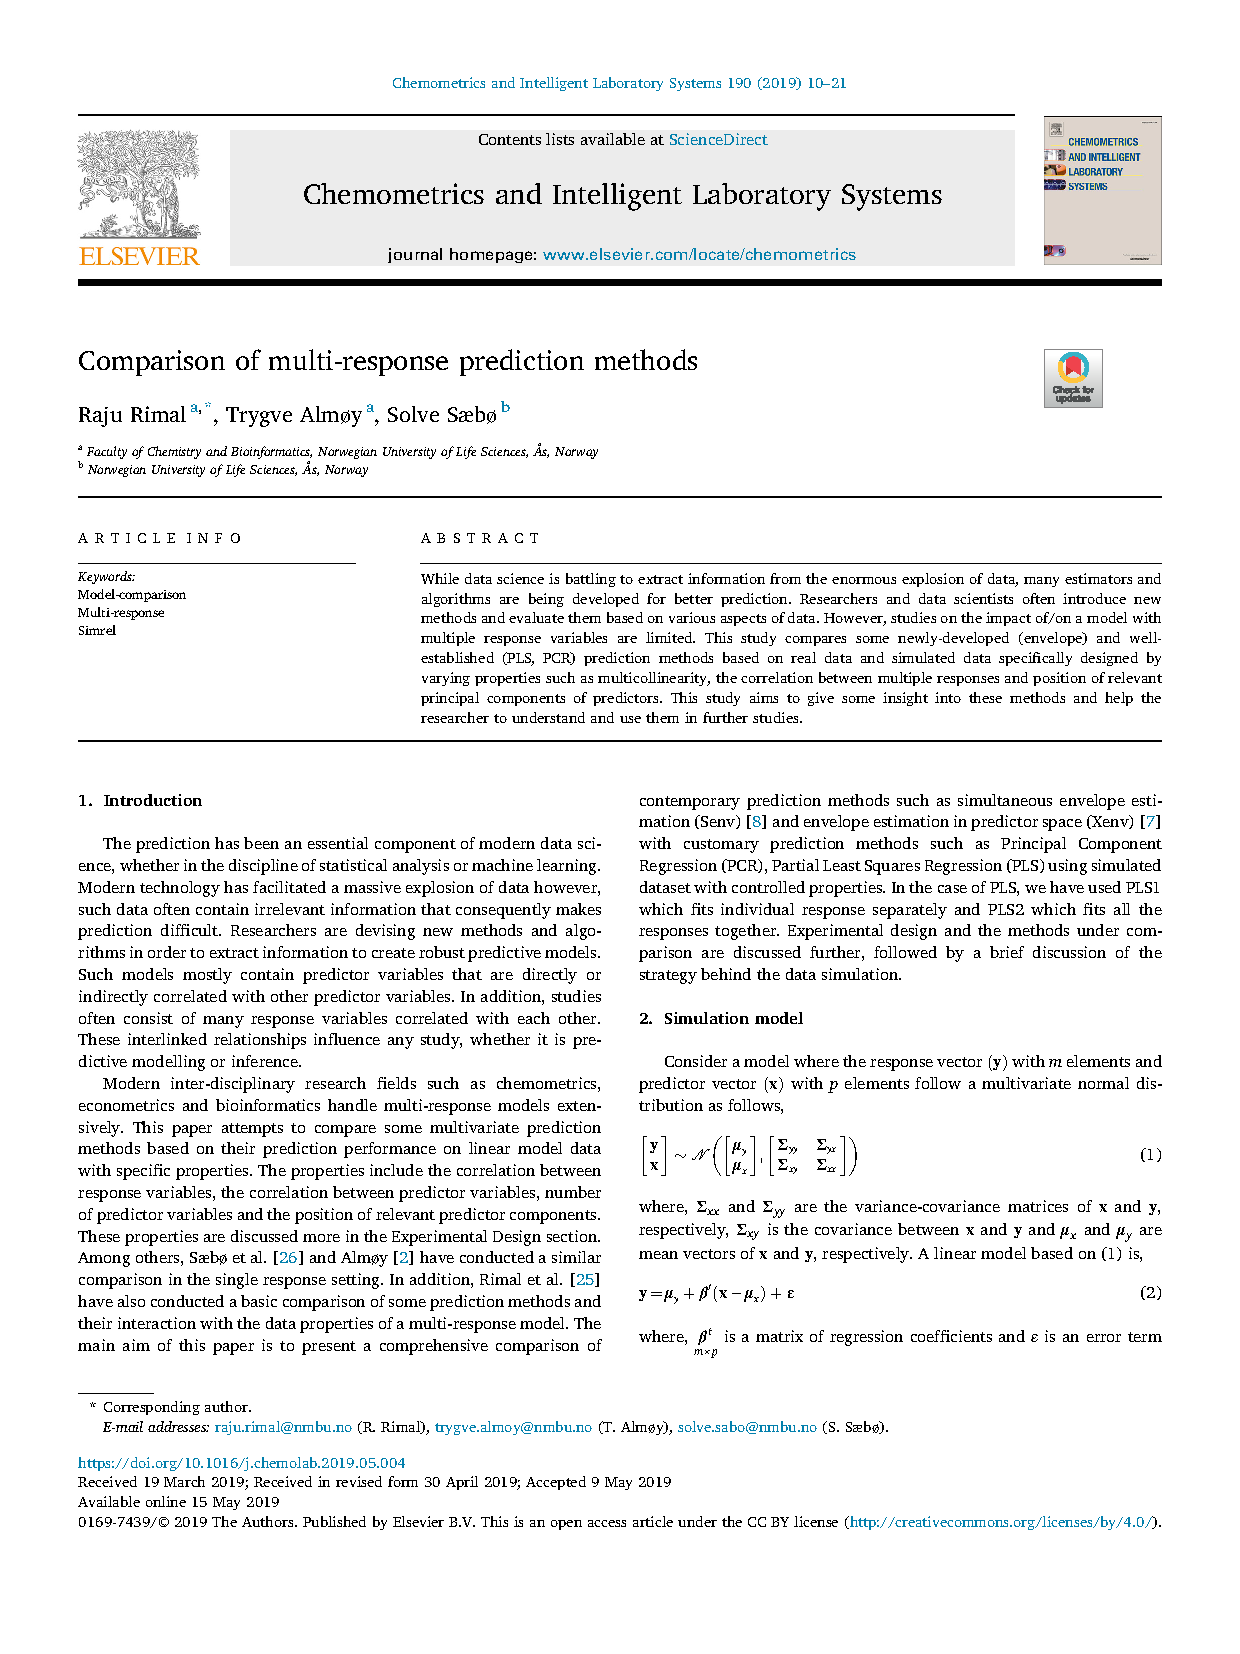
\includepdf[pages=-]{papers/003.pdf}

\end{document}
